\documentclass[../root]{subfiles}
\graphicspath{{_images/}{../_images/}}

\begin{document}

    \chapter{Social motives in birateral bargaining games: \\ How power changes perceptions of fairness}

    \begin{shortsummary}
        \begin{itemize}
            \item \authoryear{Mallucchi2019}
            \item \RQ{How does power shape the perceptions of fairness in economic interactions? Are they driven by selfish motives or act upon the belief that they deserve it.}
            \item \answer{Experimental studies using a modified ultimatum game.}
            \item \result{Changes in power can modify what is perceived as a fair decision, and thus influence the distributive behaviors and outcomes.}
        \end{itemize}
    \end{shortsummary}

    \section{Introduction}

    \paragraph{Power}

    \begin{itemize}
      \item Power is one of the most important social motivations of human behavior (Iyer and Villas Boas, 2003; Winter, 2007).
      \item Power moderates the social preferences.
      \begin{itemize}
        \item more egocentric (Galinsky et al., 2008; Guinote 2007; Keltner et al., 2003)
        \item pay less attention to others (Fiske 1993; Galinsky et al., 2006; Gruenfeld et al., 2008; Overbeck and Park 2001; Schmid Mast et al. 2009)
        \item display higher degrees of moral hypocrisy (Lammers et al., 2010)

        \ldots
      \end{itemize}
    \end{itemize}

    \paragraph{Fairness}

    \begin{itemize}
      \item Research in experimental economics has aregued that human motivation is a mix of both self-interests and other-regarding preferences: important determinants of distributive behavior and outcomes (Camerer, 2003).
      \item The perception of fair outcomes can be affected by a number of factors:
      \begin{itemize}
        \item players' efforts/contributions (Cappelen et al., 2007)
        \item skills (Cappelen et al., 2010)
        \item itentetions (Bolton et al., 2005; Charness and Rabin 2002)

        \ldots
      \end{itemize}
    \end{itemize}

    \paragraph{Setting Research Question and Approach}

    \begin{itemize}
      \item What is unclear: How power interects with fairness conerns in determining distributions.
      \item Outcome power $\equiv$ the ability of to bring out desired outcomes.

      $\Rightarrow$ Experiment to identify a direct causal relationship, and conditions.
      \item Experiment: modified bilateral ultimatum and dictator game: introduce a probability condition that endogenizes the likelihood for the second mover to be able to reject a proposal.
      \begin{itemize}
        \item within-subject design to observe a responder's choice under different choice.
        \item 2 $\times$ 2 between-subject design
        \begin{enumerate}
          \item public vs. private information for the responder of the probability
          \item feedback of information about their opponents' decision.
        \end{enumerate}
      \end{itemize}
    \end{itemize}

    \paragraph{Sum of the Results}

    \begin{itemize}
      \item Common knowledge of the power distribution between two parties constitutes a necessary condition for changes in behaviors to occur.
      \item Feedbacks from the game, in contrast, do not contribute to the main effect of probability on players’ decisions.
      \begin{itemize}
        \item Feedbacks may help subjects adjust behaviors to avoid money left on the table in negotiations
      \end{itemize}
    \end{itemize}

    \section{Literature}

    \begin{itemize}
      \item Little attention has been given to the possible interaction between power and fairness.
      \item Channel structure and roles can change the incentives of channel members as well as the power differential.
      \begin{itemize}
        \item Hsu(2008), two-person public good games: strategic concerns explain overall behavior better than fairness motives.
        \item Rustichini and Villeval (2014), dictator, ultimatum, and trust games: fairness is a compromise between self-image and monetary payoffs, an power affects the extent to which a subject adjust this judgment.
        \item Andreoni et al. (2013), convex game: the responder reduces the risk of the proposer for making more selfish offer.
      \end{itemize}
      \item More direct approach to modify the power balance.
      \begin{itemize}
        \item Suleiman (1996), exogeneous discount factor to punish the proposer.
      \end{itemize}
      \item Distributional effects using multilateral bargaining.
      \begin{itemize}
        \item Reserchers examine how distribution of proposal and veto powers influence resource allocations.
        \item Frechette et al. (2005b): nominal changes in power does not affect behaviors.
      \end{itemize}
      \item Probability-manipulation approach affects both real and mominal powers of the proposer, but the nominal power of the responder.
      \begin{itemize}
        \item Real powers: change the consequences for the game equilibrium
        \item Nominal: not
      \end{itemize}
    \end{itemize}

    \section{The modified ultimatum game}

    \begin{itemize}
      \item Proceedure
      \begin{enumerate}
        \item A fixed amount of money to split $E$ and the probability condition $\pi$ which determines if the responder's option to reject the offer.
        \item Both the responder and the proposer simultaneously determine the allocation $p$ and the threshold $t$.
      \end{enumerate}
      \item $\pi$ shifts the power differential without qualitatively changing their relationship: a convex combination of the standard dictator and ultimatum games.
    \end{itemize}


    \begin{figure}[ht]
        \centering
        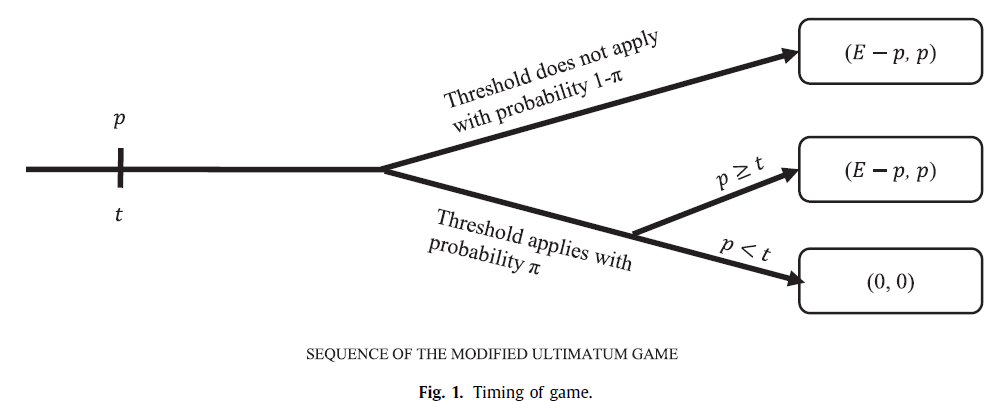
\includegraphics[scale = .8]{1106tanji/F1}
    \end{figure}

    \begin{itemize}
      \item The utility functions of the proposer $u_p$ and the responder $u_r$ are defind as
      \begin{align*}
        u_r &= \begin{cases}
          p - \alpha (m_k E - p)^+ - \beta (p - m_k E)^+ & \text{ if } p \geq t \\
          \pi * 0 + (1 - \pi) * [p - \alpha (m_k E - p)^+ - \beta (p - m_k E)^+] & \text{ if } p < t
      \end{cases} \\
      u_p &= \begin{cases}
        E - p - \alpha_p [n_k E - (E - p)]^+ - \beta_p [(E - p) - n_k E]^+ & \text{ if } p \geq t \\
        \pi * 0 + (1 - \pi) * \left\{E - p - \alpha_p [n_k E - (E - p)]^+ - \beta_p [(E - p) - n_k E]^+ \right\} & \text{ if } p < t
      \end{cases}
      \end{align*}
      \begin{itemize}
        \item $m_k, n_k, \beta \in ]0, 1[$
        \item $\alpha_p \geq \beta_p$.
      \end{itemize}
      \item Equilibrium: trembling hand perfect.
      \begin{align*}
        t^*(\alpha) &= \dfrac{\alpha}{1 + \alpha}m_k E, \\
        p^*(\alpha) &= \begin{cases}
          \dfrac{\alpha}{1 + \alpha} m_k E & \text{ if } \pi \geq \dfrac{(1 - \beta_p) \alpha}{1 + \alpha}\dfrac{m_k}{1 - \beta_p + \beta_p n_k} \\
          0 &  \text{ if } \pi < \dfrac{(1 - \beta_p) \alpha}{1 + \alpha}\dfrac{m_k}{1 - \beta_p + \beta_p n_k}
      \end{cases}
      \end{align*}
    \end{itemize}

    \begin{itembox}[l]{Proposition 1}
      A responder will modify her acceptance threshold iff her preferences for fairness are changed.
    \end{itembox}

    \begin{itembox}[l]{Proposition 2}
      There exists a breakpoint in $\pi$ for the proposer to make a non-zero offer, which is positively correlated with the responder's preferences for fairness.
    \end{itembox}

    \begin{itemize}
      \item We can vary the responder's power through the probability condition.
      \item We can elicit the responder's fairness considerations using the acceptance threshold.
    \end{itemize}


    \section{Experimental design and implementation}

    \begin{itemize}
      \item Each participants play convex game for 8 rounds.
      \item $E = 100$ experimental "pesos"
      \item The game was programmed using z-Tree (Fischbacher 2007).
      \item Subjects: undergraduates at the University of Wisconsin-Madison.
      \begin{itemize}
        \item Students cannot participate in the experiment more than once.
      \end{itemize}
      \item Fees
      \begin{itemize}
        \item Show-up fees (\$5) + about 12\$ (randomly drawn results of the 8 rounds.)
        \item An experimental session lasted 30-40 minutes.
      \end{itemize}
      \item \#participants: 128
    \end{itemize}

    \paragraph{Within-subject design}

    \begin{itemize}
      \item Each participants experiences:
      \begin{itemize}
        \item both the proposer and the responder.
        \item both low and high probability conditions ($\pi = 10\%, 90\%)$.
      \end{itemize}
      \item Each set lasts 2 in a sequence.
    \end{itemize}

    \paragraph{Between-subject design}

    \begin{itemize}
      \item 2 $\times$ 2 information types:
      \begin{enumerate}
        \item Full vs. Asymmetric information on probability conditions $\pi$
        \item Whether or not feedbacks are available per round.
        \begin{itemize}
          \item offer of the proposer
          \item threshold of the responder
          \item whether or not the threshold is executed
          \item the final split
        \end{itemize}
      \end{enumerate}

      \begin{table}
        \centering
        \begin{tabular}{lcc}\hline \hline
          info. of $\pi$ \textbackslash Feedback & Yes  & No \\ \hline
          Yes & FN & FF \\
          No & AN & AF \\ \hline \hline
        \end{tabular}

        Baseline is FN (Full information \& No feedback).
      \end{table}
    \end{itemize}

    \paragraph{Post-game Questionnaire}

    \begin{itemize}
      \item Manipulation check as to whether participants recognized the power shift.
      \item Stated fairness preferences
      \item "What-if" scenarios to check subjects' understanding of the strategic implications from common knowledge about the probability condition.
    \end{itemize}


    \section{Results}

    \subsection{Experimental results}

    \paragraph{Time trend and effect of role switch}

    \begin{itemize}
      \item Significant time trend only exists in AF treatments.
      \begin{itemize}
        \item Offers by the proposer in general decreases.
        \item Switching roles does not affect subjects' choices of either offers or thresholds.
      \end{itemize}
    \end{itemize}

    \begin{figure}[ht]
      \centering
      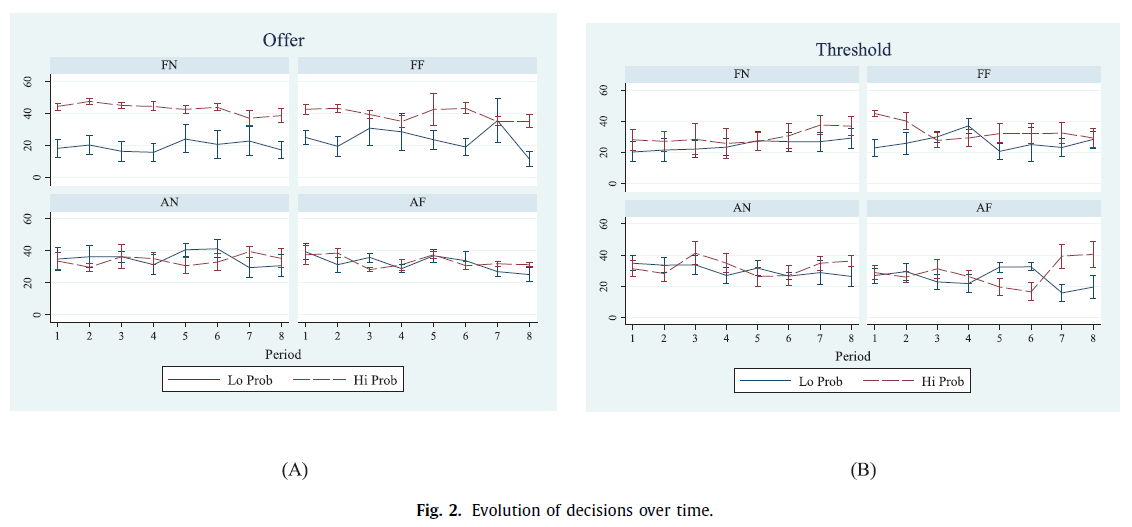
\includegraphics[scale = .8]{1106tanji/F2}
    \end{figure}

    \paragraph{Within-subject comparisons}

    \begin{itemize}
      \item Under FN, proposers offer more and responders demand more, under the high probability condition.
      \begin{itemize}
        \item Even when a change in power does not affect one's incentives directly, the responders still react to it.
      \end{itemize}
      \item Under Asymmmetric information treatment, the difference does not occur.
    \end{itemize}

    \begin{figure}[ht]
        \centering
        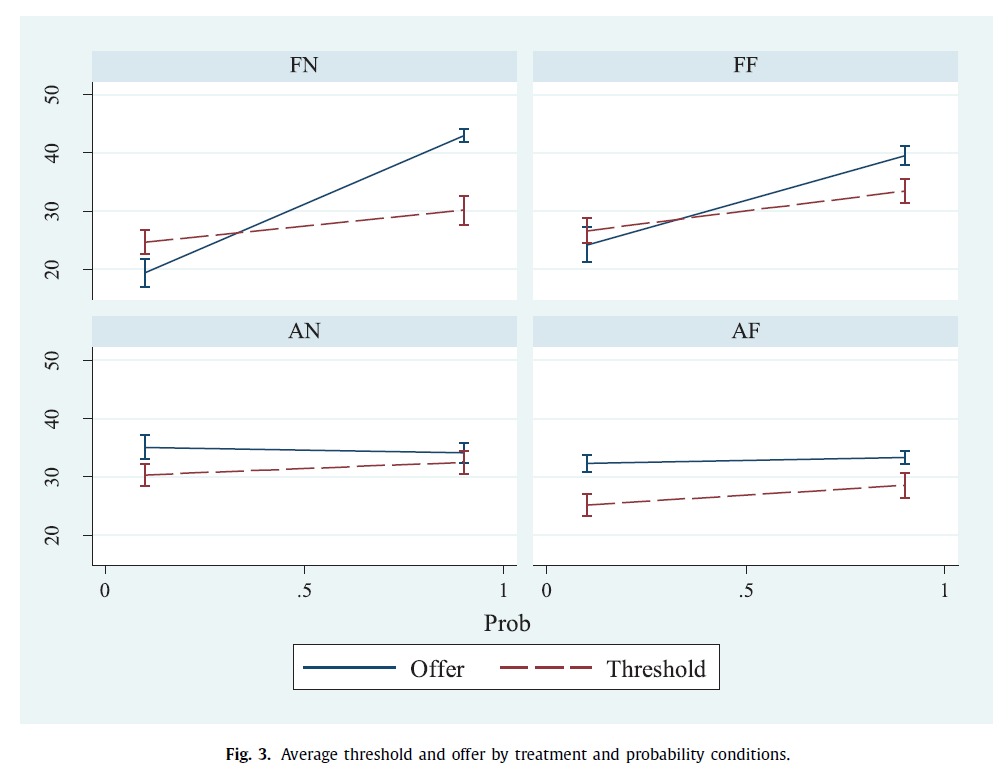
\includegraphics[scale = .8]{1106tanji/F3}
        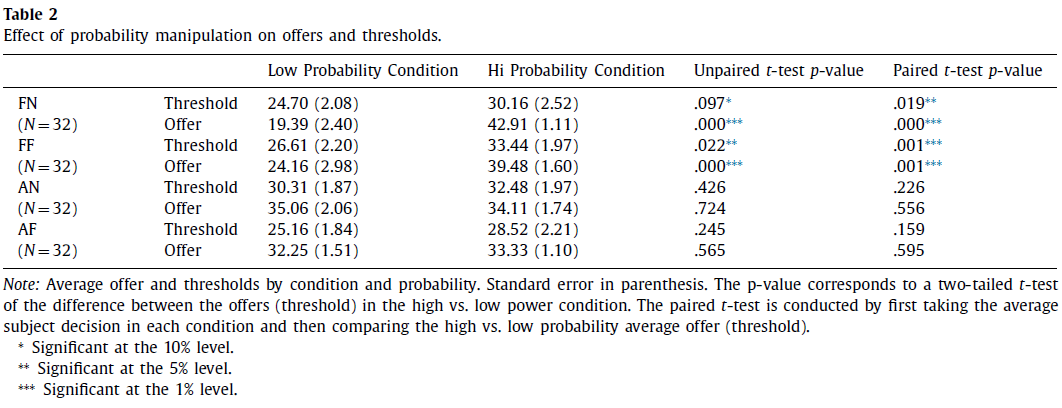
\includegraphics[scale = .8]{1106tanji/T2}
    \end{figure}

    \paragraph{Between-subject comparisons}

    \begin{itemize}
      \item The role of feedback information:
      \begin{itemize}
        \item A responder may learn to increase her threshold after observing from the past feedbacks that the proposer tends to offer more under the high probability condition, and vice versa.
      \end{itemize}
      \item Providing feedbacks per round helps reduce the absolute difference between the decisions of matched pairs.
      \begin{itemize}
        \item FF vs. FN: the absolute difference between offers \& thresholds decreases when feedback was made.
        \item AN vs.AF: threshold decreases significantly, particulary under the low probability.
      \end{itemize}
    \end{itemize}

    \subsection{Discussion of alternative explanations}

    \paragraph{Signaling and reputation building}

    \begin{itemize}
      \item Treatments without feedbacks show the same reaction by the responders.
    \end{itemize}

    \paragraph{Anchoring}

    \begin{itemize}
      \item Responders may have set higher thresholds simply because they saw a larger number(probability).
      \begin{itemize}
        \item Such effects should have occur in all the treatments.
      \end{itemize}
    \end{itemize}

    \paragraph{Experimenter demand effect}

    \begin{itemize}
      \item Subjects may have been cued to modify when they face and compare different probability.
      \begin{itemize}
        \item Such effects should have occur in all the treatments.
        \item Using only first round $\Rightarrow$ similar results.
      \end{itemize}
    \end{itemize}

    \subsection{Post survey measures}

    \begin{itemize}
      \item The probability conditions and the subjects' evaluation about the power differentials were linked.
      \item Judgements as a social planner: attributed significantly less to responders with low probability.
      \item Players prefered the treatment with more power under full information.
    \end{itemize}

    \section{Discussion and Conclusion}

    \paragraph{Contribution}

    \begin{itemize}
      \item to the literature on fairness by improving the understanding of its causes, consequences, and relationship with power.
      \begin{itemize}
        \item A change in one players incentive can trigger a change in the other player's behavior.
      \end{itemize}
      \item to the experimental design.
      \begin{itemize}
        \item Simultaneous move to control the reputation building.
        \item probability condition: convex combination of the two games.
      \end{itemize}
    \end{itemize}

    \paragraph{Implications}

    \begin{itemize}
      \item Attention to power dynamics.
      \item Perceptions of power change.
    \end{itemize}

    \paragraph{Limitaions}

    \begin{itemize}
      \item Identification of the exact cause of the power influence on the fairness: $m_k, \alpha$.
    \end{itemize}

    \paragraph{Remarks}

    \begin{itemize}
      \item Power assigned by coin toss.
      \item Extending the distribution.
    \end{itemize}


    %\begin{figure}[]
    %    \centering
    %    \includegraphics[scale = 1]{1106tanji/ignore file.txt}
    %\end{figure}

    \biblio

\end{document}
